\documentclass[]{book}
\usepackage{lmodern}
\usepackage{amssymb,amsmath}
\usepackage{ifxetex,ifluatex}
\usepackage{fixltx2e} % provides \textsubscript
\ifnum 0\ifxetex 1\fi\ifluatex 1\fi=0 % if pdftex
  \usepackage[T1]{fontenc}
  \usepackage[utf8]{inputenc}
\else % if luatex or xelatex
  \ifxetex
    \usepackage{mathspec}
  \else
    \usepackage{fontspec}
  \fi
  \defaultfontfeatures{Ligatures=TeX,Scale=MatchLowercase}
\fi
% use upquote if available, for straight quotes in verbatim environments
\IfFileExists{upquote.sty}{\usepackage{upquote}}{}
% use microtype if available
\IfFileExists{microtype.sty}{%
\usepackage{microtype}
\UseMicrotypeSet[protrusion]{basicmath} % disable protrusion for tt fonts
}{}
\usepackage{hyperref}
\hypersetup{unicode=true,
            pdftitle={Applications of Machine Learning in Imputation},
            pdfauthor={Methodology},
            pdfborder={0 0 0},
            breaklinks=true}
\urlstyle{same}  % don't use monospace font for urls
\usepackage{natbib}
\bibliographystyle{apalike}
\usepackage{color}
\usepackage{fancyvrb}
\newcommand{\VerbBar}{|}
\newcommand{\VERB}{\Verb[commandchars=\\\{\}]}
\DefineVerbatimEnvironment{Highlighting}{Verbatim}{commandchars=\\\{\}}
% Add ',fontsize=\small' for more characters per line
\usepackage{framed}
\definecolor{shadecolor}{RGB}{248,248,248}
\newenvironment{Shaded}{\begin{snugshade}}{\end{snugshade}}
\newcommand{\KeywordTok}[1]{\textcolor[rgb]{0.13,0.29,0.53}{\textbf{#1}}}
\newcommand{\DataTypeTok}[1]{\textcolor[rgb]{0.13,0.29,0.53}{#1}}
\newcommand{\DecValTok}[1]{\textcolor[rgb]{0.00,0.00,0.81}{#1}}
\newcommand{\BaseNTok}[1]{\textcolor[rgb]{0.00,0.00,0.81}{#1}}
\newcommand{\FloatTok}[1]{\textcolor[rgb]{0.00,0.00,0.81}{#1}}
\newcommand{\ConstantTok}[1]{\textcolor[rgb]{0.00,0.00,0.00}{#1}}
\newcommand{\CharTok}[1]{\textcolor[rgb]{0.31,0.60,0.02}{#1}}
\newcommand{\SpecialCharTok}[1]{\textcolor[rgb]{0.00,0.00,0.00}{#1}}
\newcommand{\StringTok}[1]{\textcolor[rgb]{0.31,0.60,0.02}{#1}}
\newcommand{\VerbatimStringTok}[1]{\textcolor[rgb]{0.31,0.60,0.02}{#1}}
\newcommand{\SpecialStringTok}[1]{\textcolor[rgb]{0.31,0.60,0.02}{#1}}
\newcommand{\ImportTok}[1]{#1}
\newcommand{\CommentTok}[1]{\textcolor[rgb]{0.56,0.35,0.01}{\textit{#1}}}
\newcommand{\DocumentationTok}[1]{\textcolor[rgb]{0.56,0.35,0.01}{\textbf{\textit{#1}}}}
\newcommand{\AnnotationTok}[1]{\textcolor[rgb]{0.56,0.35,0.01}{\textbf{\textit{#1}}}}
\newcommand{\CommentVarTok}[1]{\textcolor[rgb]{0.56,0.35,0.01}{\textbf{\textit{#1}}}}
\newcommand{\OtherTok}[1]{\textcolor[rgb]{0.56,0.35,0.01}{#1}}
\newcommand{\FunctionTok}[1]{\textcolor[rgb]{0.00,0.00,0.00}{#1}}
\newcommand{\VariableTok}[1]{\textcolor[rgb]{0.00,0.00,0.00}{#1}}
\newcommand{\ControlFlowTok}[1]{\textcolor[rgb]{0.13,0.29,0.53}{\textbf{#1}}}
\newcommand{\OperatorTok}[1]{\textcolor[rgb]{0.81,0.36,0.00}{\textbf{#1}}}
\newcommand{\BuiltInTok}[1]{#1}
\newcommand{\ExtensionTok}[1]{#1}
\newcommand{\PreprocessorTok}[1]{\textcolor[rgb]{0.56,0.35,0.01}{\textit{#1}}}
\newcommand{\AttributeTok}[1]{\textcolor[rgb]{0.77,0.63,0.00}{#1}}
\newcommand{\RegionMarkerTok}[1]{#1}
\newcommand{\InformationTok}[1]{\textcolor[rgb]{0.56,0.35,0.01}{\textbf{\textit{#1}}}}
\newcommand{\WarningTok}[1]{\textcolor[rgb]{0.56,0.35,0.01}{\textbf{\textit{#1}}}}
\newcommand{\AlertTok}[1]{\textcolor[rgb]{0.94,0.16,0.16}{#1}}
\newcommand{\ErrorTok}[1]{\textcolor[rgb]{0.64,0.00,0.00}{\textbf{#1}}}
\newcommand{\NormalTok}[1]{#1}
\usepackage{longtable,booktabs}
\usepackage{graphicx,grffile}
\makeatletter
\def\maxwidth{\ifdim\Gin@nat@width>\linewidth\linewidth\else\Gin@nat@width\fi}
\def\maxheight{\ifdim\Gin@nat@height>\textheight\textheight\else\Gin@nat@height\fi}
\makeatother
% Scale images if necessary, so that they will not overflow the page
% margins by default, and it is still possible to overwrite the defaults
% using explicit options in \includegraphics[width, height, ...]{}
\setkeys{Gin}{width=\maxwidth,height=\maxheight,keepaspectratio}
\IfFileExists{parskip.sty}{%
\usepackage{parskip}
}{% else
\setlength{\parindent}{0pt}
\setlength{\parskip}{6pt plus 2pt minus 1pt}
}
\setlength{\emergencystretch}{3em}  % prevent overfull lines
\providecommand{\tightlist}{%
  \setlength{\itemsep}{0pt}\setlength{\parskip}{0pt}}
\setcounter{secnumdepth}{5}
% Redefines (sub)paragraphs to behave more like sections
\ifx\paragraph\undefined\else
\let\oldparagraph\paragraph
\renewcommand{\paragraph}[1]{\oldparagraph{#1}\mbox{}}
\fi
\ifx\subparagraph\undefined\else
\let\oldsubparagraph\subparagraph
\renewcommand{\subparagraph}[1]{\oldsubparagraph{#1}\mbox{}}
\fi

%%% Use protect on footnotes to avoid problems with footnotes in titles
\let\rmarkdownfootnote\footnote%
\def\footnote{\protect\rmarkdownfootnote}

%%% Change title format to be more compact
\usepackage{titling}

% Create subtitle command for use in maketitle
\providecommand{\subtitle}[1]{
  \posttitle{
    \begin{center}\large#1\end{center}
    }
}

\setlength{\droptitle}{-2em}

  \title{Applications of Machine Learning in Imputation}
    \pretitle{\vspace{\droptitle}\centering\huge}
  \posttitle{\par}
    \author{Methodology}
    \preauthor{\centering\large\emph}
  \postauthor{\par}
      \predate{\centering\large\emph}
  \postdate{\par}
    \date{2019}

\usepackage{booktabs}
\usepackage{amsthm}
\makeatletter
\def\thm@space@setup{%
  \thm@preskip=8pt plus 2pt minus 4pt
  \thm@postskip=\thm@preskip
}
\makeatother

\begin{document}
\maketitle

{
\setcounter{tocdepth}{1}
\tableofcontents
}
\chapter{Introduction}\label{introduction}

Editing and imputation are both methods of data processing. Editing
refers to the detection and correction of errors in the data, whilst
imputation is a method of correcting errors in a dataset \citep{deWaal}.
This document presents findings from work carried out at the Office for
National Statistics on the use of machine learning in imputation. The
chapters address the following questions:

\begin{enumerate}
\def\labelenumi{\arabic{enumi})}
\tightlist
\item
  What is imputation?\\
\item
  What is machine learning?\\
\item
  Why use machine learning?\\
\item
  How XGBoost works?\\
\item
  Methods used for the investigation\\
\item
  Results of the investigation\\
\item
  Conclusions and future direction
\end{enumerate}

\chapter{What is Imputation?}\label{what-is-imputation}

Editing and imputing are both methods of data processing. Editing refers
to the detection and correction of errors in the data. Whilst imputation
is a method of correcting errors and estimating and filling in missing
values in a dataset. Where there are errors in the dataset, and when
these are considered to add no value in the correction process, these
values are set to missing and are imputed with a plausible estimate.
Alternatively, missing values may already exist in the data, and
imputation may be carried out to produce a complete dataset for
analysis.

This research project evaluated the use of machine learning methods for
imputation. In order to provide a context for using machine learning in
the imputation process, the reader is presented with:

\begin{itemize}
\tightlist
\item
  A rationale for carrying out imputation\\
\item
  An introduction to the methods of imputation
\end{itemize}

\section{Why is imputation carried
out?}\label{why-is-imputation-carried-out}

Missingness and erroneous values can impact the quality of data. A large
volume of incorrect and/or missing values increase the risk of the
product failing to capture the target concept or target population. That
is, ommissions (introduced in collection or processing) may result in
certain sub-groups of the target population from being excluded in the
analysis dataset, and in turn increasing the risk of biased estimates,
reducing the power of inferential statistics and increasing the
uncertainty of estimates and inferences derived from the data.
Similarly, errors in a dataset may impact the degree to which the final
estimate or output represents the reality it was designed to capture.

Correcting erroneous responses and filling in missing values helps
manage the quality of data. A complete dataset can improve the accuracy
and reliability of estimates, and help maintain the consistency of
counts across published tables. Moreover, a dataset with fewer errors
and more units may more accuately capture the underlying distribution of
the variable of interest. Selecting a method for estimating values in a
datset is generally advised by the nature of errors or missingness in
the data, and the output desired from the analysis dataset.

\section{Methods}\label{methods}

An imputation process of a dataset can be broken down into the following
three phases:

\begin{enumerate}
\def\labelenumi{\arabic{enumi})}
\tightlist
\item
  Review, whereby data is examined for potential problems; identifying
  instances of missingness and erroneous values\\
\item
  Select, whereby data is identified for further treatment. Of the
  potential problems identified in the review phase, a method is applied
  to determine which of these erroneous or missing cases need to be
  treated
\item
  Amend, whereby changes are applied to the data identified in the
  select phase by either correcting errors/ filling in missing values
\end{enumerate}

The focus of this project was in applying Machine Learning methods to
amend values in a dataset. That is, it was of interest to compare
existing approaches, of treating missing or erroneous values by
estimating replacement figures, to machine learning methods. Methods of
variable amendment can be grouped into one of the following categories:

\begin{itemize}
\tightlist
\item
  interactive treatment\\
\item
  deductive imputation\\
\item
  model based imputation\\
\item
  donor based imputation
\end{itemize}

The mechanisms for a given imputation method could be deterministic or
stochastic. The former refers to instances where repeated trials of the
same method yield identical output. Whereas the latter refers to
instances where there is element of randomness; repeated iterations will
produce different results.

\subsection{Interactive treatment}\label{interactive-treatment}

Interactive treatment refers to a class of methods whereby the data are
adjusted by a human editor by either re-contacting the respondent/ data
provider, replacing values from another variable/ data source, or
creating a value based on subject matter expertise.

\subsection{Deductive imputation}\label{deductive-imputation}

Deductive imputation uses logic or an understanding about the
relationship between variables and units to fill in missing values.
Examples include deriving a value as a function of other values,
adopting a value from a related unit, and adopting a value from an
earlier time point. Generally, this method is used when the true value
can be derived with certainty or with a very high probability.

\subsection{Model based imputation}\label{model-based-imputation}

Model based imputation refers to a class of methods that estimate
missing values using assumptions about the distribution of the data,
which include mean and median imputation. Or assumptions about the
relationship between auxiliary variables (or x variables) and the target
y variable to predict missing values.

\subsection{Donor based imputation}\label{donor-based-imputation}

Donor based imputation adopt values from an observed unit, which are
then used for the missing unit. For each recipient with a missing value
for variable y, a donor is identified that is similar to the recipient
with respect to certain background characteristics (often referred to as
matching variables) that are related to the target variable y. Such
methods are relatively easy to apply when there are several related
missing values in one record, and if the intention is to preserve the
relationship between variables.

\chapter{What is Machine Learning?}\label{what-is-machine-learning}

Machine learning is the field of study that enables a program to learn
from its experience of iterating through a task multiple times. A
performance measure is generally specified by the programmer, which is
used to evaluate how well the machine has carried out the task at each
iteration. Learning of the task is evidenced by its improvement against
the performance measure.\\
The different types of machine learning systems can be categorised with
respect to:

\begin{itemize}
\tightlist
\item
  Whether or not they are trained with human supervision\\
\item
  Whether or not they can learn incrementally or on the fly\\
\item
  Whether they work by comparing new data points to known data points,
  or instead detect patterns in the training data and build a predictive
  model
\end{itemize}

\section{Supervision}\label{supervision}

Machine learning systems can vary with regards to the degree of
supervision. The major types of supervision:

\begin{itemize}
\tightlist
\item
  Supervised learning\\
\item
  Unsupervised learning\\
\item
  Semi-supervised learning\\
\item
  Reinforcement learning
\end{itemize}

\subsection{Supervised learning}\label{supervised-learning}

Supervised learning is the specification of the desired output. That is,
the data used to train the model includes the solutions (which are
referred to as labels), which the machine learning system attempts to
estimate. The desired solutions specified in the machine learning
algorithm are referred to as labels.

\subsection{Unsupervised learning}\label{unsupervised-learning}

Unsupervised learning uses training data that is unlabelled. In this
class of machine learning systems, the outcome/ desired solutions are
not specified in the machine learning algorithm.

\subsection{Semi-supervised learning}\label{semi-supervised-learning}

Machine learning systems that use partially labelled data are
categorised as utilising semi-supervised learning.

\subsection{Reinforcement learning}\label{reinforcement-learning}

Reinforcement learning involves the use of rewards or penalties to train
the machine in identifying the appropriate action for a given situation.
The learning system, which is referred to as an agent, observes the
environment, selects and performs actions, and gets a response in the
form of a reward or penalty. After multiple iterations, it identifies
the best strategy, referred to as a policy, that results in the most
reward over time.

\section{Batch and Online learning}\label{batch-and-online-learning}

Another criterion for classifying machine learning systems is the way in
which the algorithm learns. That is, whether the learning takes place at
once or if it happens in increments.

\subsection{Batch learning}\label{batch-learning}

Batch learning uses all the available data to train the machine learning
system. This is generally time consuming and computationally expensive,
and as a result is carried out offline. Whilst in production, the system
is no longer learning, and is simply applying what it has learnt from
the full set of training data.

Any changes to the data generating mechanism (GDM) will mean that a new
system would need to be trained, from scratch on the full set of data
(that includes data points before and after changes to the GDM).

\subsection{Online learning}\label{online-learning}

Online learning trains the system incrementally through sequential input
of data. Data can be delivered individually or in small groups, referred
to as mini-batches. As each learning step is relatively fast and cheap,
the system can learn about new data whilst in production, as it arrives.
It is an ideal approach for when the velocity of new data is high, and
when there is a need to adapt to changes rapidly or autonomously.

\section{Approaches to
generalisation}\label{approaches-to-generalisation}

Machine learning systems can also be categorised with regards to how the
systems generalise. That is, there are different approaches to using the
training data to develop a system that can then be generalised to new
cases. The two main approaches are instance-based learning and
model-based learning.

\subsection{Instance-based learning}\label{instance-based-learning}

Instance-based learning identifies all instances of a given feature in
the training data and uses a similarity measure to generalise to new
cases.

\subsection{Model-based learning}\label{model-based-learning}

Model-based learning uses features in the training data to predict the
outcome/ variable of interest; the model used to specify the
relationship between the predictor(s) and outcome(s) are then
generalised on new cases.

\chapter{Why use Machine Learning?}\label{why-use-machine-learning}

It was of interest to explore the utility of Machine Learning to
directly impute for missing values in datasets. More specifically, the
Methods Division was interested in examining whether Machine Learning
models can improve the timeliness, reliability and accuracy of the
imputation process in social survey data. Figure 1 presents the
imputation pipeline for social survey data. Prior to imputation, units
and values are reviewed, and those that are missing and should be routed
to the item in question, are selected (i.e.~flagged) for imputation.
Data is then further processed by the Social Survey Division before
imputed and observed data are compiled in an analysis dataset, used for
publishing Official Statistics estimates.

\begin{figure}
\centering
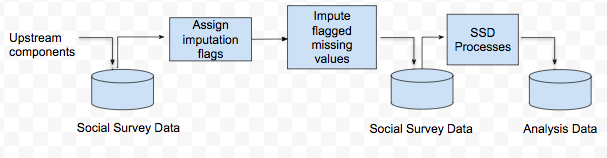
\includegraphics{images/CurrentPipeline.png}
\caption{Figure 1. Imputation pipeline in social survey data.}
\end{figure}

The intention was to use a machine learning system to impute flagged
missing values. This model based approach for imputation may reduce the
data processing time and improve the precision and reduce the variance
of estimates. The current approach, which utilises nearest neighbour
donor imputation involves the following:

\begin{itemize}
\tightlist
\item
  Setting up specification files for each variable and imputation group
  combination\\
\item
  Iterating through weights for matching variables so that all missing
  values are imputed
\end{itemize}

Designing the selection criteria for donors can be time consuming as it
requires analysts to identify matching variables (MV), along with
weights for each MV. Teams currently use subject matter expertise in
designing the donor imputation strategy for each variable. As this
process is not data driven, it introduces an element of subjectivity and
does not guarantee that matching variables selected are the best
predictors of the variable of interest. In contrast, a data driven
approach would be reproducible and identify the best predictors, in the
dataset, to estimate missing values. Moreover, applying the machine
learning system may offer a more parsimonious approach as fewer input
paramters and files would be required in executing imputation.

The Methodology Division was interested in whether a Machine Learning
System would perform better compared to the current imputation process
with regards to:

\begin{itemize}
\tightlist
\item
  Timeliness: Would the ML system reduce processing time and by how
  much?\\
\item
  Accuracy \& Reliability: How do the two methods compare with respect
  to the bias and variance of estimates?\\
\item
  Interpretability: What advantages and challenges do the ML system
  present with regards to making the imputation methods transparent?
\end{itemize}

The following Machine Learning tools were used in the investigation:

\begin{itemize}
\tightlist
\item
  XGBoost\\
\item
  Generative Adverserial Networks\\
\item
  Autoencoder
\end{itemize}

\chapter{XGBoost}\label{xgboost}

XGBoost is a set of open source functions and steps, referred to as a
library, that use supervised ML where analysts specify an outcome to be
estiamted/ predicted. The XGBoost library uses multiple decision trees
to predict an outcome.

The ML system is trained using batch learning and generalised through a
model based approach. It uses all available data to construct a model
that specifies the relationship between the predictor and outcome
variables, which are then generalised on the test data.

XGBoost stands for eXtreme Gradient Boosting. The word ``extreme''
reflects its goal to push the limit of computational resources. Whereas
gradient boosting is a machine learning technique for regression and
classification problems that optimises a collection of weak prediction
models in an attempt to build an accurate and reliable predictor.

In order to build a better understanding of how XGBoost works, the
documentation will briefly review:

\begin{itemize}
\tightlist
\item
  Decision trees\\
\item
  Boosting\\
\item
  Regularisation
\end{itemize}

\section{Decision trees}\label{decision-trees}

Decision trees can be used as a method for grouping units in a dataset
by asking questions, such as ``Does an individual have a Bachelor's
degree?''. In this example, two groups would be created; one for those
with a Bachelor's degree, and one for those without. Figure 2 provides a
visual depiction of this grouping in an attempt to explain Income.

\begin{figure}
\centering
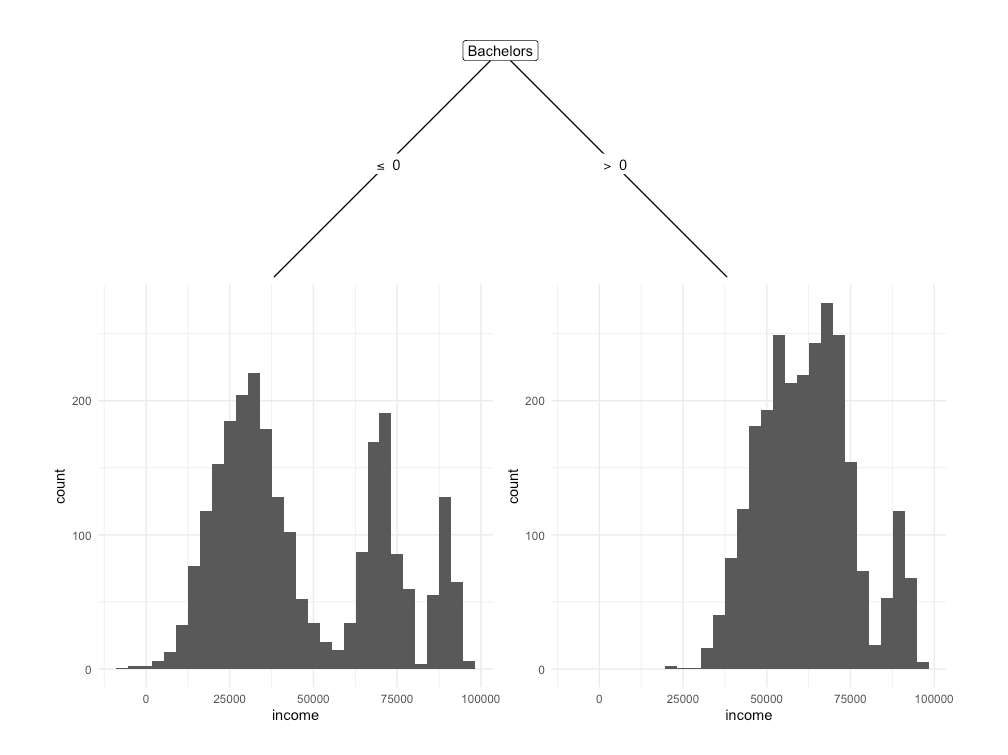
\includegraphics{images/dt_bach.png}
\caption{Figure 2. Decision tree that splits units in a dataset based on
whether individual has a Bachelor's degree or not, in order to predict
Income. The tree shows that those with a Bachelors degree on average
earn more than than those wihtout a Bachelor's degree.}
\end{figure}

Each subsequent question in a decision tree will produce a smaller group
of units. This grouping is carried out to identify units with similar
characteristics with respect to an outcome variable. The model in Figure
3 attempts to use University qualifications to predict Income.

\begin{figure}
\centering
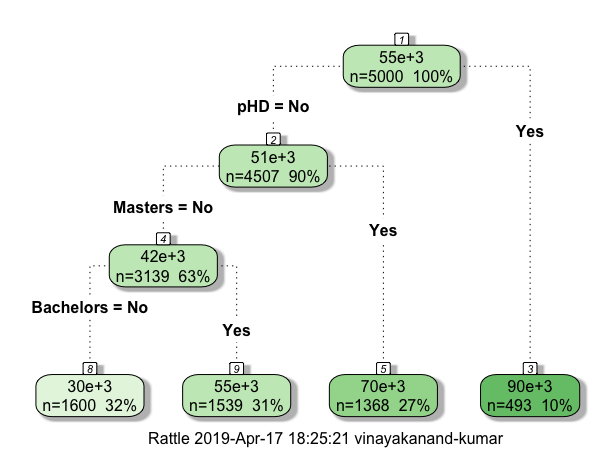
\includegraphics{images/dt_all.png}
\caption{Figure 3. Decision tree that splits units in a dataset based on
whether individual has a Bachelor's degree (yes/no), a Master's degree
and pHD (yes/no), in order to predict Income. The tree shows that those
with a higher qualification tend to earn more.}
\end{figure}

The following characteristics are true of decision trees:

\begin{itemize}
\tightlist
\item
  A single question is asked at each decision node, and there are only
  two possible choices. With the example in Figure 3, the questions
  include 1) Does individual have a pHD, 2) Does individual have a
  Master's and 3) Does individual have a Bachelor's degree.\\
\item
  At the bottom of every decision tree, there is a single possible
  decision. Every possible decision will eventually lead to a choice.
  Some decisions will lead to a choice sooner. The model in Figure 3
  attempts to predict Income using University Qualifications. Each node
  presents the average income, size and percentage composition for a
  given subset of the dataset. The end nodes present the average income
  for individuals with the specified qualifications. As a result, the
  choices would be the expected value of Income for an individual, given
  the qualificaitons obtained.
\end{itemize}

Decision trees are a learning method that involve a tree like graph to
model either continuous or categorical choice given some data. It is
composed of a series of binary questions, which when answered in
succession yield a prediciton about data at hand. XGBoost uses
Classification and Regression Trees (CART), which are presented in the
above examples, to predict the outcome variable.

\subsection{Boosting}\label{boosting}

A single decision tree is considered a weak/ base learner as it only
slightly better than chance at predicting the outcome variable. Whereas
strong learners are any algorithm that can be tuned to achieve peak
performance for supervised learning. XGBoost uses decision trees as base
learners; combining many weak learners to form a strong learner. As a
result it is referred to as an ensemble learning method; using the
output of many models (i.e.~trees) in the final prediction.

The concept of combining many weak learners to produce a strong learner
is referred as boosting. XGBoost will iteratively build a set of weak
models on subsets of the data; weighting each weak prediction according
to the weak learner's performance. A prediction is derived by taking the
weighted sum of all base learners.

\subsection{Building models with
XGBoost}\label{building-models-with-xgboost}

In the training data, a target variable \(y_{i}\) is specified, whilst
all other features \(x_{i}\) are used as predictors of the target
variable. A collection of decision trees are used to predict values of
\(y_{i}\) using \(x_{i}\). Individually, each decision tree, would be a
weak predictor of the outcome variable. However, as a collective, the
decision trees may enable analysts to make accurate and reliable
predictions of \(y_{i}\). As a result, the method for predicting the
target variable using \(x_{i}\) in XGBoost is referred to as decision
tree ensembles. The steps below demonstrate how XGBoost was used to
build a model, to predict income, using Univeristy Qualifications.

\begin{enumerate}
\def\labelenumi{\arabic{enumi})}
\tightlist
\item
  Load the following packages
\end{enumerate}

\begin{Shaded}
\begin{Highlighting}[]
\KeywordTok{library}\NormalTok{(caret)}
\KeywordTok{library}\NormalTok{(xgboost)}
\end{Highlighting}
\end{Shaded}

\begin{enumerate}
\def\labelenumi{\arabic{enumi})}
\setcounter{enumi}{1}
\tightlist
\item
  Load the dataset and remove the identifer
\end{enumerate}

\begin{Shaded}
\begin{Highlighting}[]
\NormalTok{#### Load data #### }
\KeywordTok{load}\NormalTok{(}\StringTok{"data/Income_tree.RData"}\NormalTok{)}

\NormalTok{#### Remove identifier ####}
\NormalTok{Income <-}\StringTok{ }\NormalTok{Income[,}\OperatorTok{-}\DecValTok{1}\NormalTok{]}
\end{Highlighting}
\end{Shaded}

\begin{enumerate}
\def\labelenumi{\arabic{enumi})}
\setcounter{enumi}{2}
\tightlist
\item
  Split the dataset into training and test
\end{enumerate}

\begin{Shaded}
\begin{Highlighting}[]
\NormalTok{#### Split data into training and test ####}
\KeywordTok{set.seed}\NormalTok{(}\DecValTok{5}\NormalTok{)}
\NormalTok{s <-}\StringTok{ }\KeywordTok{createDataPartition}\NormalTok{(Income}\OperatorTok{$}\NormalTok{income, }\DataTypeTok{p =} \FloatTok{0.8}\NormalTok{, }\DataTypeTok{list=}\OtherTok{FALSE}\NormalTok{)}
\NormalTok{training <-}\StringTok{ }\NormalTok{Income[s,]}
\NormalTok{test <-}\StringTok{ }\NormalTok{Income[}\OperatorTok{-}\NormalTok{s,]}
\end{Highlighting}
\end{Shaded}

\begin{enumerate}
\def\labelenumi{\arabic{enumi})}
\setcounter{enumi}{3}
\tightlist
\item
  Convert the data into DMatrix objects, which is the recommended input
  type for xgboost
\end{enumerate}

\begin{Shaded}
\begin{Highlighting}[]
\NormalTok{#### Convert the data to a matrix and assign output variable first ####}
\NormalTok{train.outcome <-}\StringTok{ }\NormalTok{training}\OperatorTok{$}\NormalTok{income}
\NormalTok{train.predictors <-}\StringTok{ }\KeywordTok{sparse.model.matrix}\NormalTok{(income }\OperatorTok{~}\StringTok{ }\NormalTok{.,}
                                        \DataTypeTok{data =}\NormalTok{ training}
\NormalTok{)[, }\OperatorTok{-}\DecValTok{1}\NormalTok{]}
\NormalTok{test.outcome <-}\StringTok{ }\NormalTok{test}\OperatorTok{$}\NormalTok{income}
\NormalTok{test.predictors <-}\StringTok{ }\KeywordTok{model.matrix}\NormalTok{(income }\OperatorTok{~}\StringTok{ }\NormalTok{.,}
                                \DataTypeTok{data =}\NormalTok{ test}
\NormalTok{)[, }\OperatorTok{-}\DecValTok{1}\NormalTok{]}

\NormalTok{#### Convert the matrix objects to DMatrix objects ####}
\NormalTok{dtrain <-}\StringTok{ }\KeywordTok{xgb.DMatrix}\NormalTok{(train.predictors, }\DataTypeTok{label=}\NormalTok{train.outcome)}
\NormalTok{dtest <-}\StringTok{ }\KeywordTok{xgb.DMatrix}\NormalTok{(test.predictors)}
\end{Highlighting}
\end{Shaded}

\begin{enumerate}
\def\labelenumi{\arabic{enumi})}
\setcounter{enumi}{4}
\tightlist
\item
  Train the model
\end{enumerate}

\begin{Shaded}
\begin{Highlighting}[]
\NormalTok{#### Train the model ####}
\NormalTok{model <-}\StringTok{ }\KeywordTok{xgboost}\NormalTok{(}
  \DataTypeTok{data =}\NormalTok{ dtrain, }\DataTypeTok{max_depth =} \DecValTok{2}\NormalTok{, }\DataTypeTok{eta =} \DecValTok{1}\NormalTok{, }\DataTypeTok{nthread =} \DecValTok{2}\NormalTok{, }\DataTypeTok{nrounds =} \DecValTok{10}\NormalTok{,}
  \DataTypeTok{objective =} \StringTok{"reg:linear"}\NormalTok{)}
\end{Highlighting}
\end{Shaded}

\begin{enumerate}
\def\labelenumi{\arabic{enumi})}
\setcounter{enumi}{5}
\tightlist
\item
  Test the model
\end{enumerate}

\begin{Shaded}
\begin{Highlighting}[]
\NormalTok{#### Test the model ####}
\NormalTok{pred <-}\StringTok{ }\KeywordTok{predict}\NormalTok{(model, dtest)}

\NormalTok{#### Evaluate the performance of model ####}
\KeywordTok{RMSE}\NormalTok{(pred,test.outcome)}
\end{Highlighting}
\end{Shaded}

\begin{enumerate}
\def\labelenumi{\arabic{enumi})}
\setcounter{enumi}{6}
\tightlist
\item
  Examine the importance of each feature in the model
\end{enumerate}

\begin{Shaded}
\begin{Highlighting}[]
\NormalTok{#### Examine feature importance ####}
\NormalTok{importance_matrix <-}\StringTok{ }\KeywordTok{xgb.importance}\NormalTok{(}\DataTypeTok{model =}\NormalTok{ model)}
\KeywordTok{print}\NormalTok{(importance_matrix)}
\KeywordTok{xgb.plot.importance}\NormalTok{(}\DataTypeTok{importance_matrix =}\NormalTok{ importance_matrix)}
\end{Highlighting}
\end{Shaded}

\begin{enumerate}
\def\labelenumi{\arabic{enumi})}
\setcounter{enumi}{7}
\tightlist
\item
  Plot the individual trees in the model
\end{enumerate}

\begin{Shaded}
\begin{Highlighting}[]
\CommentTok{# Tree 1}
\KeywordTok{xgb.plot.tree}\NormalTok{(}\DataTypeTok{model =}\NormalTok{ model, }\DataTypeTok{tree=}\DecValTok{0}\NormalTok{)}
\CommentTok{# Tree 2}
\KeywordTok{xgb.plot.tree}\NormalTok{(}\DataTypeTok{model =}\NormalTok{ model, }\DataTypeTok{tree=}\DecValTok{1}\NormalTok{)}
\CommentTok{# Tree 3}
\KeywordTok{xgb.plot.tree}\NormalTok{(}\DataTypeTok{model =}\NormalTok{ model, }\DataTypeTok{tree=}\DecValTok{2}\NormalTok{)}
\end{Highlighting}
\end{Shaded}

\chapter{Methods}\label{methods-1}

The project evaluated the machine learning methods using:\\
1) The Census Teaching File, an open dataset containing 1\% of the
person records from the 2011 Census in England \& Wales.\\
2) Survey Data

The code below specifies the packages used in the preparation, study and
build of machine learning systems using the Census Teaching File.

\begin{Shaded}
\begin{Highlighting}[]
\KeywordTok{library}\NormalTok{(tidyverse)}
\KeywordTok{library}\NormalTok{(mice)}
\KeywordTok{library}\NormalTok{(reshape2)}
\KeywordTok{library}\NormalTok{(GGally)}
\KeywordTok{library}\NormalTok{(Matrix)}
\KeywordTok{library}\NormalTok{(xgboost)}
\KeywordTok{library}\NormalTok{(caret)}
\KeywordTok{library}\NormalTok{(DiagrammeR)}
\KeywordTok{library}\NormalTok{(MLmetrics)}
\KeywordTok{library}\NormalTok{(rpart)}
\KeywordTok{library}\NormalTok{(scales)}
\KeywordTok{library}\NormalTok{(knitr)}
\KeywordTok{library}\NormalTok{(kableExtra)}
\KeywordTok{library}\NormalTok{(DescTools)}
\end{Highlighting}
\end{Shaded}

\section{Census Teaching File}\label{census-teaching-file}

The Census Teaching File was downloaded from the
\href{https://www.ons.gov.uk/census/2011census/2011censusdata/censusmicrodata/microdatateachingfile}{ONS
website} as a CSV file named ``CensusTeachingFile'', and was read into R
using the following line of code. The dataset consisted of 569,741
individuals and 18 categorical variables from the 2011 Census
population.

\begin{Shaded}
\begin{Highlighting}[]
\CommentTok{# Read CSV into R}
\NormalTok{CensusRaw <-}\StringTok{ }\KeywordTok{read.csv}\NormalTok{(}
  \DataTypeTok{file =} \StringTok{"Data/CensusTeachingFile.csv"}\NormalTok{, }\DataTypeTok{skip =} \DecValTok{1}\NormalTok{,}
  \DataTypeTok{header =} \OtherTok{TRUE}\NormalTok{, }\DataTypeTok{sep =} \StringTok{","}
\NormalTok{)}
\end{Highlighting}
\end{Shaded}

Variables in the dataset were renamed and recoded so that:

\begin{itemize}
\tightlist
\item
  Variable names were consisted with
  \href{https://google.github.io/styleguide/Rguide.xml}{Google's R style
  guide}
\item
  The response categories for all variables were numeric
\end{itemize}

\begin{Shaded}
\begin{Highlighting}[]
\CommentTok{# Rename variables}
\NormalTok{Census <-}\StringTok{ }\NormalTok{plyr}\OperatorTok{::}\KeywordTok{rename}\NormalTok{(CensusRaw, }\KeywordTok{c}\NormalTok{(}
  \StringTok{"Person.ID"}\NormalTok{ =}\StringTok{ "person.id"}\NormalTok{,}
  \StringTok{"Region"}\NormalTok{ =}\StringTok{ "region"}\NormalTok{,}
  \StringTok{"Residence.Type"}\NormalTok{ =}\StringTok{ "residence.type"}\NormalTok{,}
  \StringTok{"Family.Composition"}\NormalTok{ =}\StringTok{ "fam.comp"}\NormalTok{,}
  \StringTok{"Population.Base"}\NormalTok{ =}\StringTok{ "resident.type"}\NormalTok{,}
  \StringTok{"Sex"}\NormalTok{=}\StringTok{"sex"}\NormalTok{,}
  \StringTok{"Age"}\NormalTok{=}\StringTok{"age"}\NormalTok{,}
  \StringTok{"Marital.Status"}\NormalTok{ =}\StringTok{ "marital.status"}\NormalTok{,}
  \StringTok{"Student"}\NormalTok{=}\StringTok{"student"}\NormalTok{,}
  \StringTok{"Country.of.Birth"}\NormalTok{ =}\StringTok{ "birth.country"}\NormalTok{,}
  \StringTok{"Health"}\NormalTok{=}\StringTok{"health"}\NormalTok{,}
  \StringTok{"Ethnic.Group"}\NormalTok{ =}\StringTok{ "ethnicity"}\NormalTok{,}
  \StringTok{"Religion"}\NormalTok{=}\StringTok{"religion"}\NormalTok{,}
  \StringTok{"Economic.Activity"}\NormalTok{ =}\StringTok{ "econ.act"}\NormalTok{,}
  \StringTok{"Occupation"}\NormalTok{ =}\StringTok{ "occupation"}\NormalTok{,}
  \StringTok{"Industry"}\NormalTok{ =}\StringTok{ "industry"}\NormalTok{,}
  \StringTok{"Hours.worked.per.week"}\NormalTok{ =}\StringTok{ "hours.worked"}\NormalTok{,}
  \StringTok{"Approximated.Social.Grade"}\NormalTok{ =}\StringTok{ "social.grade"}
\NormalTok{))}

\CommentTok{# Recode variables (dataset is mutated in order to recode variables)}
\NormalTok{Census <-}\StringTok{ }\NormalTok{Census }\OperatorTok\StringTok{ }\KeywordTok{mutate_if}\NormalTok{(is.factor, as.character)}

\CommentTok{# Recode the Region variable so that it is numeric}
\NormalTok{Census}\OperatorTok{$}\NormalTok{region[Census}\OperatorTok{$}\NormalTok{region }\OperatorTok{==}\StringTok{ "E12000001"}\NormalTok{] <-}\StringTok{ }\DecValTok{1}
\NormalTok{Census}\OperatorTok{$}\NormalTok{region[Census}\OperatorTok{$}\NormalTok{region }\OperatorTok{==}\StringTok{ "E12000002"}\NormalTok{] <-}\StringTok{ }\DecValTok{2}
\NormalTok{Census}\OperatorTok{$}\NormalTok{region[Census}\OperatorTok{$}\NormalTok{region }\OperatorTok{==}\StringTok{ "E12000003"}\NormalTok{] <-}\StringTok{ }\DecValTok{3}
\NormalTok{Census}\OperatorTok{$}\NormalTok{region[Census}\OperatorTok{$}\NormalTok{region }\OperatorTok{==}\StringTok{ "E12000004"}\NormalTok{] <-}\StringTok{ }\DecValTok{4}
\NormalTok{Census}\OperatorTok{$}\NormalTok{region[Census}\OperatorTok{$}\NormalTok{region }\OperatorTok{==}\StringTok{ "E12000005"}\NormalTok{] <-}\StringTok{ }\DecValTok{5}
\NormalTok{Census}\OperatorTok{$}\NormalTok{region[Census}\OperatorTok{$}\NormalTok{region }\OperatorTok{==}\StringTok{ "E12000006"}\NormalTok{] <-}\StringTok{ }\DecValTok{6}
\NormalTok{Census}\OperatorTok{$}\NormalTok{region[Census}\OperatorTok{$}\NormalTok{region }\OperatorTok{==}\StringTok{ "E12000007"}\NormalTok{] <-}\StringTok{ }\DecValTok{7}
\NormalTok{Census}\OperatorTok{$}\NormalTok{region[Census}\OperatorTok{$}\NormalTok{region }\OperatorTok{==}\StringTok{ "E12000008"}\NormalTok{] <-}\StringTok{ }\DecValTok{8}
\NormalTok{Census}\OperatorTok{$}\NormalTok{region[Census}\OperatorTok{$}\NormalTok{region }\OperatorTok{==}\StringTok{ "E12000009"}\NormalTok{] <-}\StringTok{ }\DecValTok{9}
\NormalTok{Census}\OperatorTok{$}\NormalTok{region[Census}\OperatorTok{$}\NormalTok{region }\OperatorTok{==}\StringTok{ "W92000004"}\NormalTok{] <-}\StringTok{ }\DecValTok{10}

\NormalTok{Census}\OperatorTok{$}\NormalTok{residence.type[Census}\OperatorTok{$}\NormalTok{residence.type }\OperatorTok{==}\StringTok{ "C"}\NormalTok{] <-}\StringTok{ }\DecValTok{1}
\NormalTok{Census}\OperatorTok{$}\NormalTok{residence.type[Census}\OperatorTok{$}\NormalTok{residence.type }\OperatorTok{==}\StringTok{ "H"}\NormalTok{] <-}\StringTok{ }\DecValTok{2}

\NormalTok{Census}\OperatorTok{$}\NormalTok{student[Census}\OperatorTok{$}\NormalTok{student }\OperatorTok{==}\StringTok{ }\DecValTok{1}\NormalTok{] <-}\StringTok{ }\DecValTok{0}
\NormalTok{Census}\OperatorTok{$}\NormalTok{student[Census}\OperatorTok{$}\NormalTok{student }\OperatorTok{==}\StringTok{ }\DecValTok{2}\NormalTok{] <-}\StringTok{ }\DecValTok{1}

\NormalTok{Census <-}\StringTok{ }\NormalTok{Census }\OperatorTok\StringTok{ }\KeywordTok{mutate_if}\NormalTok{(is.character, as.numeric)}

\NormalTok{Census}\OperatorTok{$}\NormalTok{person.id <-}\StringTok{ }\KeywordTok{as.character}\NormalTok{(Census}\OperatorTok{$}\NormalTok{person.id)}

\NormalTok{Ht <-}\StringTok{ }\KeywordTok{table}\NormalTok{(Census}\OperatorTok{$}\NormalTok{hours.worked)}
\NormalTok{Census}\OperatorTok{$}\NormalTok{hours.cont <-}\StringTok{ }\KeywordTok{ifelse}\NormalTok{(Census}\OperatorTok{$}\NormalTok{hours.worked }\OperatorTok{==}\StringTok{ }\DecValTok{1}\NormalTok{, }\KeywordTok{runif}\NormalTok{(}
  \DecValTok{1}\OperatorTok{:}\NormalTok{Ht[}\KeywordTok{names}\NormalTok{(Ht) }\OperatorTok{==}\StringTok{ }\DecValTok{1}\NormalTok{],}
  \DecValTok{1}\NormalTok{, }\DecValTok{15}
\NormalTok{),}
\KeywordTok{ifelse}\NormalTok{(Census}\OperatorTok{$}\NormalTok{hours.worked }\OperatorTok{==}\StringTok{ }\DecValTok{2}\NormalTok{, }\KeywordTok{runif}\NormalTok{(}\DecValTok{1}\OperatorTok{:}\NormalTok{Ht[}\KeywordTok{names}\NormalTok{(Ht) }\OperatorTok{==}\StringTok{ }\DecValTok{2}\NormalTok{], }\DecValTok{16}\NormalTok{, }\DecValTok{30}\NormalTok{),}
  \KeywordTok{ifelse}\NormalTok{(Census}\OperatorTok{$}\NormalTok{hours.worked }\OperatorTok{==}\StringTok{ }\DecValTok{3}\NormalTok{, }\KeywordTok{runif}\NormalTok{(}\DecValTok{1}\OperatorTok{:}\NormalTok{Ht[}\KeywordTok{names}\NormalTok{(Ht) }\OperatorTok{==}\StringTok{ }\DecValTok{3}\NormalTok{], }\DecValTok{31}\NormalTok{, }\DecValTok{48}\NormalTok{),}
    \KeywordTok{ifelse}\NormalTok{(Census}\OperatorTok{$}\NormalTok{hours.worked }\OperatorTok{==}\StringTok{ }\DecValTok{4}\NormalTok{, }\KeywordTok{runif}\NormalTok{(}\DecValTok{1}\OperatorTok{:}\NormalTok{Ht[}\KeywordTok{names}\NormalTok{(Ht) }\OperatorTok{==}\StringTok{ }\DecValTok{4}\NormalTok{], }\DecValTok{49}\NormalTok{, }\DecValTok{60}\NormalTok{),}
\NormalTok{      Census}\OperatorTok{$}\NormalTok{hours.worked}
\NormalTok{    )}
\NormalTok{  )}
\NormalTok{)}
\NormalTok{)}

\KeywordTok{save}\NormalTok{(Census, }\DataTypeTok{file =} \StringTok{"data/Census.Rda"}\NormalTok{)}
\end{Highlighting}
\end{Shaded}

A preview of the dataset is provided below.

\begin{verbatim}
##   person.id region residence.type fam.comp resident.type sex age
## 1   7394816      1              2        2             1   2   6
## 2   7394745      1              2        5             1   1   4
## 3   7395066      1              2        3             1   2   4
## 4   7395329      1              2        3             1   2   2
## 5   7394712      1              2        3             1   1   5
## 6   7394750      1              2        2             1   1   6
##   marital.status student birth.country health ethnicity religion econ.act
## 1              2       1             1      2         1        2        5
## 2              1       1             1      1         1        2        1
## 3              1       1             1      1         1        1        1
## 4              1       1             1      2         1        2        1
## 5              4       1             1      1         1        2        1
## 6              2       1             1      2         1        1        1
##   occupation industry hours.worked social.grade hours.cont
## 1          8        2           -9            4   -9.00000
## 2          8        6            4            3   56.92578
## 3          6       11            3            4   36.79397
## 4          7        7            3            2   36.28146
## 5          1        4            3            2   41.81308
## 6          9        2            3            3   39.98968
\end{verbatim}

For the purposes of training and testing a machine learning system, the
data was divided into training and test datasets using the following
code.

\begin{Shaded}
\begin{Highlighting}[]
\CommentTok{# Randomly select 80% of Census units and split into Train and Test data}
\KeywordTok{set.seed}\NormalTok{(}\DecValTok{5}\NormalTok{)}
\NormalTok{Census80 <-}\StringTok{ }\KeywordTok{sample}\NormalTok{(}\DecValTok{1}\OperatorTok{:}\KeywordTok{nrow}\NormalTok{(Census), }\FloatTok{0.8} \OperatorTok{*}\StringTok{ }\KeywordTok{nrow}\NormalTok{(Census), }\DataTypeTok{replace =} \OtherTok{FALSE}\NormalTok{)}
\NormalTok{Census20 <-}\StringTok{ }\KeywordTok{setdiff}\NormalTok{(}\DecValTok{1}\OperatorTok{:}\KeywordTok{nrow}\NormalTok{(Census), Census80)}

\NormalTok{Census.train <-}\StringTok{ }\NormalTok{Census[Census80, ]}
\NormalTok{Census.test <-}\StringTok{ }\NormalTok{Census[Census20, ]}

\KeywordTok{save}\NormalTok{(Census.train, }\DataTypeTok{file =} \StringTok{"data/Census.train.Rda"}\NormalTok{)}
\KeywordTok{save}\NormalTok{(Census.test, }\DataTypeTok{file =} \StringTok{"data/Census.test.Rda"}\NormalTok{)}
\end{Highlighting}
\end{Shaded}

The intention was to build models to predict each variable (listed in
Table 1) using training data, which had no missingness. This model would
then be evaluated with respect to its accuracy and generalisability
using a test dataset, which would have missingness. The Census Teaching
File was a complete dataset. As a result, missingness was simulated in
the test dataset, and the imputation models (derived for each variable)
were evaluated with regards to how well they predicted the true values.

Table 1. Variables to impute in Census Teaching File

\begin{figure}
\centering
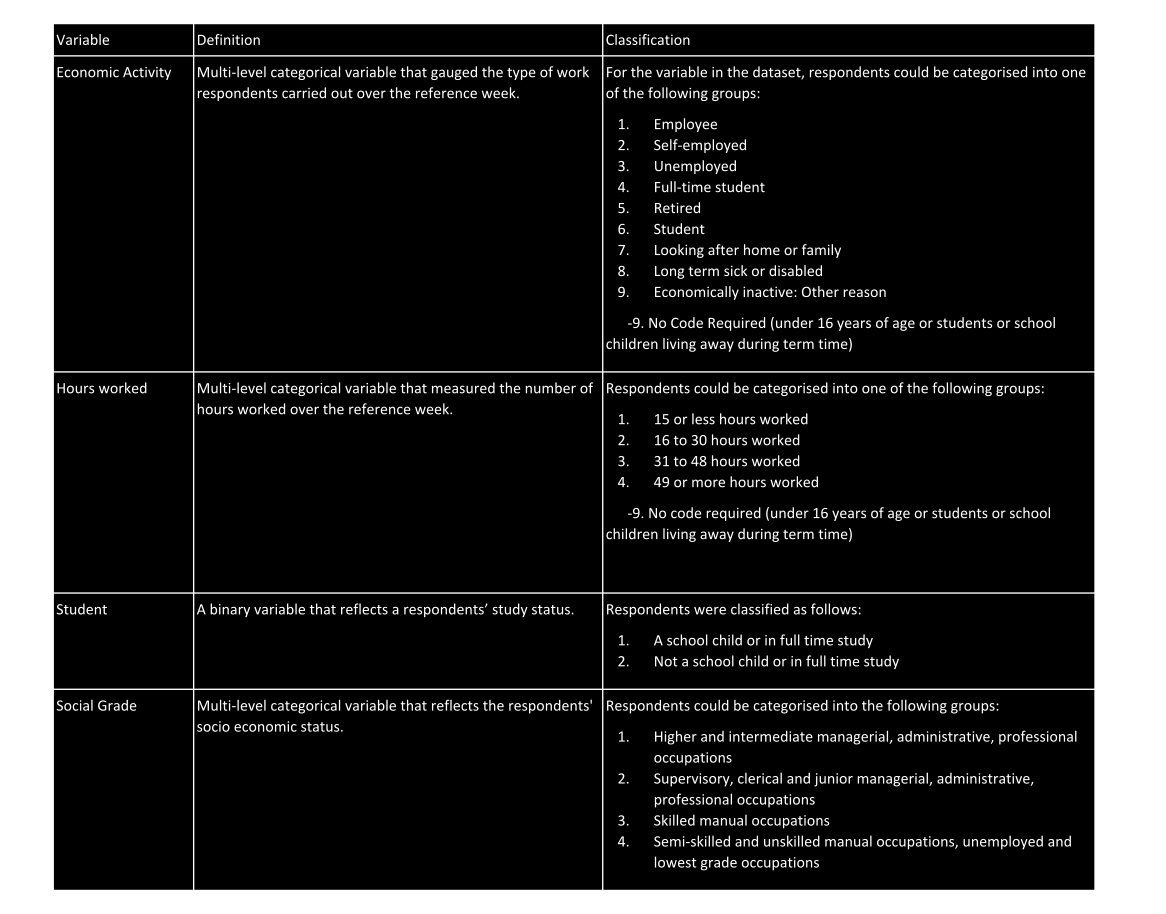
\includegraphics{images/ImputableVariables.svg}
\caption{}
\end{figure}

\chapter{Results}\label{results}

Summary statistics were produced to review the pattern of responses of
individuals included in the dataset. Please note, that all comments that
refer to respondents reflect only the respondents included in the 2011
Census Teaching File, and not descriptive statistics for the Census
Population as a whole. Summary statistics produced using the dataset
show that:

\begin{itemize}
\tightlist
\item
  The majority of respondents resided in the South East and London. A
  relatively small proportion reside in North East and Wales.\\
\item
  Almost all respondents resided in a non-communal establishment\\
\item
  The majority of respondents were living in a family that was composed
  of a married or same-sex civil partnership couple\\
\item
  Almost all respondents were usual residents at the collection address
  during time of collection\\
\item
  There were a similar number of male and female respondents in the
  dataset\\
\item
  The majority of respondents were aged 0 to 15\\
\item
  The majority of respondents were single and had never married or
  registered for a same-sex civil partnership
\item
  The majority of respondents were not school children nor were they in
  full time study
\item
  The majority of respondents were born in the United Kingdom\\
\item
  The majority of respondents reported as being in very good health at
  time of collection
\item
  With respect to Ethnicity, the majority of respondents identified as
  White\\
\item
  With respect to religion, the majority of respondents identified as
  Christian. The second largest group were those that stated they had no
  religion.\\
\item
  The two most prevalent categories for economic activity were employee
  and retired\\
\item
  Of those that were eligible to answer the Occupation item, the
  majority were either in a Professional or Elementary occupation
\item
  Of those that were eligible to answer the Industry item, the majority
  were employed in the Wholesale and retail trade industry\\
\item
  Of those that were eligible to answer the hours worked item, the
  majority worked between 31 and 38 hours per week\\
\item
  Of those elgible to answer the Social Grade item, the majority would
  be classed into the Supervisory, Clerical, and Junior Managerial
  social group
\end{itemize}

\begin{Shaded}
\begin{Highlighting}[]
\CommentTok{# Study the data: 1) How many units, 2) How many attributes? and }
\CommentTok{# 3) How many missing units?}
\KeywordTok{str}\NormalTok{(Census)}
\KeywordTok{summary}\NormalTok{(Census)}
\KeywordTok{sapply}\NormalTok{(}\KeywordTok{apply}\NormalTok{(Census[, }\KeywordTok{c}\NormalTok{(}\OperatorTok{-}\DecValTok{1}\NormalTok{, }\OperatorTok{-}\DecValTok{19}\NormalTok{)], }\DecValTok{2}\NormalTok{, table), }\ControlFlowTok{function}\NormalTok{(x) x }\OperatorTok{/}\StringTok{ }\KeywordTok{sum}\NormalTok{(x))}
\NormalTok{missing_values <-}\StringTok{ }\KeywordTok{sapply}\NormalTok{(Census, }\ControlFlowTok{function}\NormalTok{(y) }\KeywordTok{sum}\NormalTok{(}\KeywordTok{length}\NormalTok{(}\KeywordTok{which}\NormalTok{(}\KeywordTok{is.na}\NormalTok{(y)))))}
\NormalTok{missing_values <-}\StringTok{ }\KeywordTok{data.frame}\NormalTok{(missing_values)}

\CommentTok{# Look for relationship between variables}
\KeywordTok{ggcorr}\NormalTok{(Census[, }\OperatorTok{-}\DecValTok{1}\NormalTok{],}
       \DataTypeTok{nbreaks =} \DecValTok{8}\NormalTok{, }\DataTypeTok{palette =} \StringTok{"RdGy"}\NormalTok{,}
       \DataTypeTok{label =} \OtherTok{TRUE}\NormalTok{, }\DataTypeTok{label_size =} \DecValTok{3}\NormalTok{, }\DataTypeTok{label_color =} \StringTok{"white"}
\NormalTok{)}
\end{Highlighting}
\end{Shaded}

Bar charts were used to review the distribution of responses for each
categorical variable in the complete, training and test datasets (see
Figures 2 to 4). As expected, there was a similar response pattern for a
each variable between the complete, training and test datasets. The
correlation matrix in Figure 5 presents the relationship between the
variables in the complete dataset.

\begin{Shaded}
\begin{Highlighting}[]
\CommentTok{# Compare the test and training datasets}
\KeywordTok{str}\NormalTok{(Census.train)}
\KeywordTok{str}\NormalTok{(Census.test)}
\KeywordTok{summary}\NormalTok{(Census.train)}
\KeywordTok{summary}\NormalTok{(Census.test)}
\KeywordTok{sapply}\NormalTok{(}\KeywordTok{apply}\NormalTok{(Census.train[, }\KeywordTok{c}\NormalTok{(}\OperatorTok{-}\DecValTok{1}\NormalTok{, }\OperatorTok{-}\DecValTok{19}\NormalTok{)], }\DecValTok{2}\NormalTok{, table), }\ControlFlowTok{function}\NormalTok{(x) x }\OperatorTok{/}\StringTok{ }\KeywordTok{sum}\NormalTok{(x))}
\KeywordTok{sapply}\NormalTok{(}\KeywordTok{apply}\NormalTok{(Census.test[, }\KeywordTok{c}\NormalTok{(}\OperatorTok{-}\DecValTok{1}\NormalTok{, }\OperatorTok{-}\DecValTok{19}\NormalTok{)], }\DecValTok{2}\NormalTok{, table), }\ControlFlowTok{function}\NormalTok{(x) x }\OperatorTok{/}\StringTok{ }\KeywordTok{sum}\NormalTok{(x))}

\CommentTok{# Plot distribution of variables}
\NormalTok{melt.Census <-}\StringTok{ }\KeywordTok{melt}\NormalTok{(Census)}
\KeywordTok{head}\NormalTok{(melt.Census)}
\KeywordTok{ggplot}\NormalTok{(}\DataTypeTok{data =}\NormalTok{ melt.Census, }\KeywordTok{aes}\NormalTok{(}\DataTypeTok{x =}\NormalTok{ value)) }\OperatorTok{+}
\StringTok{  }\KeywordTok{geom_bar}\NormalTok{() }\OperatorTok{+}
\StringTok{  }\KeywordTok{facet_wrap}\NormalTok{(}\OperatorTok{~}\NormalTok{variable, }\DataTypeTok{scales =} \StringTok{"free"}\NormalTok{)}

\CommentTok{# Plot distribution of variables}
\NormalTok{melt.Census.train <-}\StringTok{ }\KeywordTok{melt}\NormalTok{(Census.train)}
\KeywordTok{head}\NormalTok{(melt.Census.train)}
\KeywordTok{ggplot}\NormalTok{(}\DataTypeTok{data =}\NormalTok{ melt.Census.train, }\KeywordTok{aes}\NormalTok{(}\DataTypeTok{x =}\NormalTok{ value)) }\OperatorTok{+}
\StringTok{  }\KeywordTok{geom_bar}\NormalTok{() }\OperatorTok{+}
\StringTok{  }\KeywordTok{facet_wrap}\NormalTok{(}\OperatorTok{~}\NormalTok{variable, }\DataTypeTok{scales =} \StringTok{"free"}\NormalTok{)}
\NormalTok{melt.Census.test <-}\StringTok{ }\KeywordTok{melt}\NormalTok{(Census.test)}
\KeywordTok{head}\NormalTok{(melt.Census.test)}
\KeywordTok{ggplot}\NormalTok{(}\DataTypeTok{data =}\NormalTok{ melt.Census.test, }\KeywordTok{aes}\NormalTok{(}\DataTypeTok{x =}\NormalTok{ value)) }\OperatorTok{+}
\StringTok{  }\KeywordTok{geom_bar}\NormalTok{() }\OperatorTok{+}
\StringTok{  }\KeywordTok{facet_wrap}\NormalTok{(}\OperatorTok{~}\NormalTok{variable, }\DataTypeTok{scales =} \StringTok{"free"}\NormalTok{)}
\end{Highlighting}
\end{Shaded}

\begin{figure}
\centering
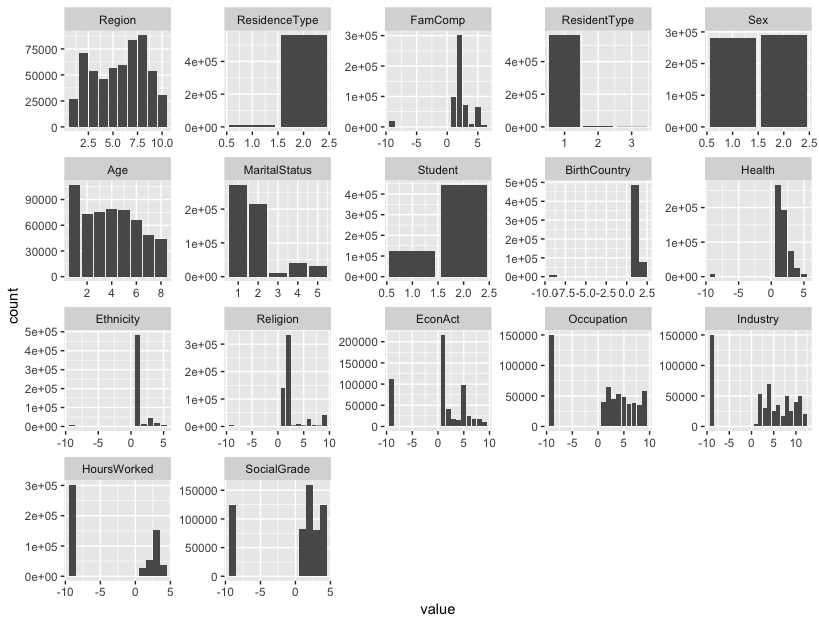
\includegraphics{images/dist_all.png}
\caption{Figure 2. Distribution of responses for variables in complete
Census Teaching File}
\end{figure}

\begin{figure}
\centering
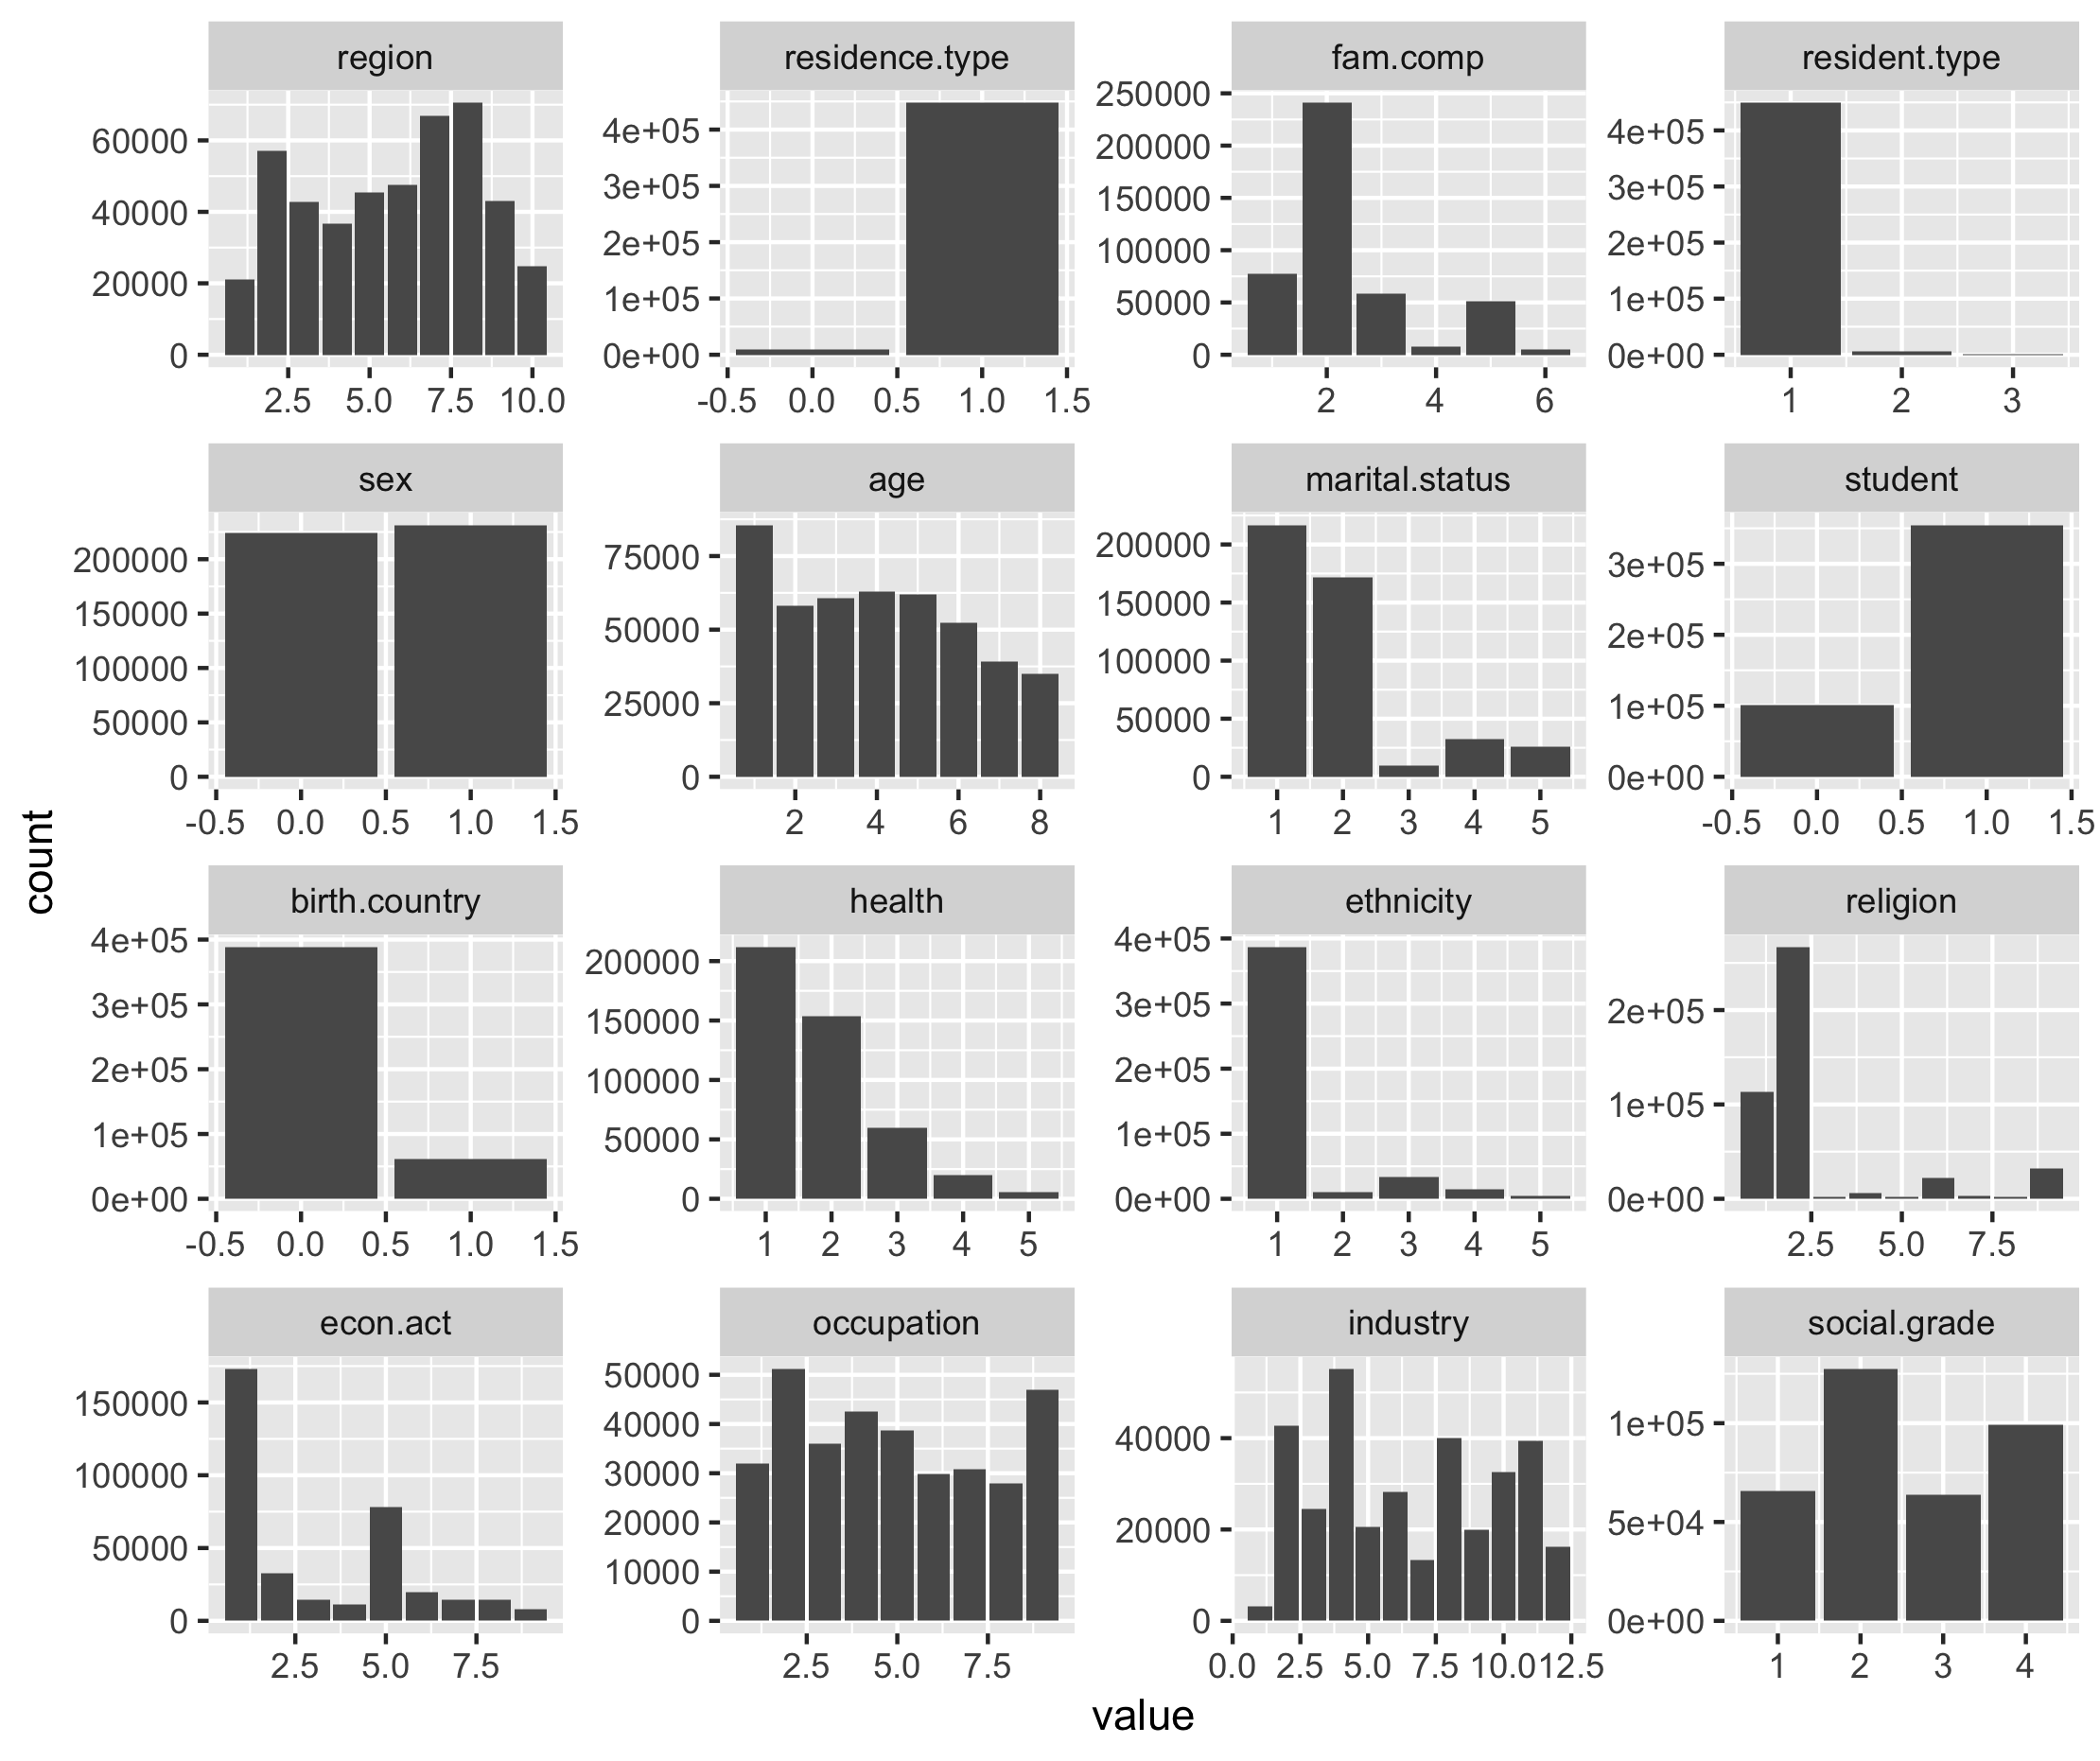
\includegraphics{images/dist_train.png}
\caption{Figure 3. Distribution of responses for variables in training
dataset}
\end{figure}

\begin{figure}
\centering
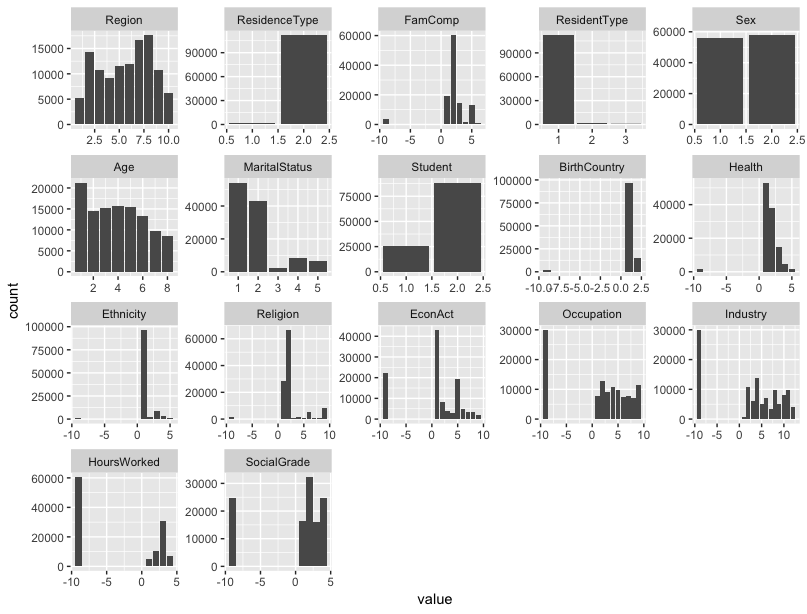
\includegraphics{images/dist_test.png}
\caption{Figure 4. Distribution of responses for variables in test
dataset}
\end{figure}

\begin{figure}
\centering
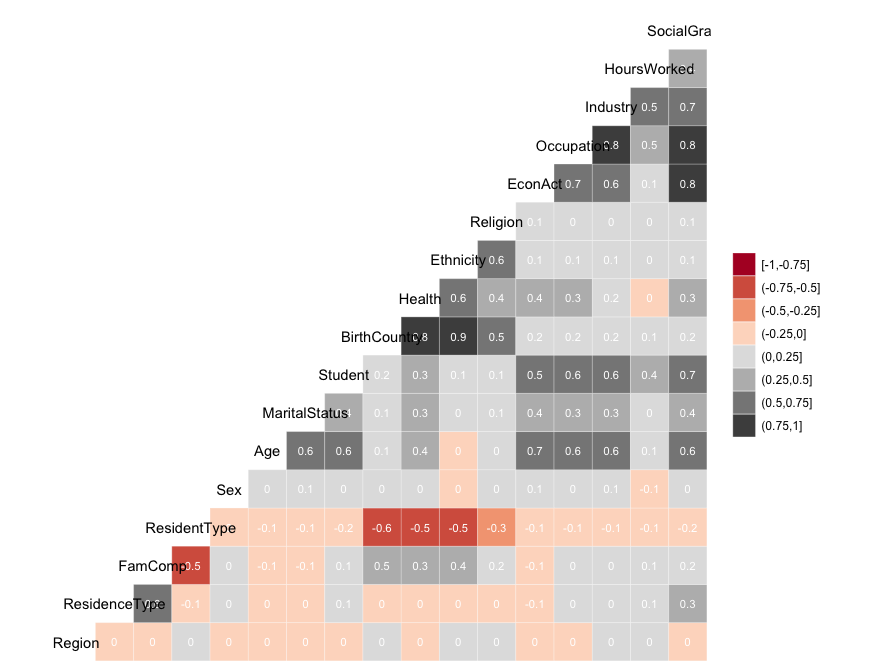
\includegraphics{images/corr_all.png}
\caption{Figure 5. Correlation matrix of variables in the Census
dataset}
\end{figure}

\chapter{Results}\label{results-1}

\section{Economic Activity}\label{economic-activity}

\section{Hours worked}\label{hours-worked}

\section{Social Grade}\label{social-grade}

\section{Student}\label{student}

\bibliography{book.bib,packages.bib}


\end{document}
